\documentclass[1p]{elsarticle_modified}
%\bibliographystyle{elsarticle-num}

%\usepackage[colorlinks]{hyperref}
%\usepackage{abbrmath_seonhwa} %\Abb, \Ascr, \Acal ,\Abf, \Afrak
\usepackage{amsfonts}
\usepackage{amssymb}
\usepackage{amsmath}
\usepackage{amsthm}
\usepackage{scalefnt}
\usepackage{amsbsy}
\usepackage{kotex}
\usepackage{caption}
\usepackage{subfig}
\usepackage{color}
\usepackage{graphicx}
\usepackage{xcolor} %% white, black, red, green, blue, cyan, magenta, yellow
\usepackage{float}
\usepackage{setspace}
\usepackage{hyperref}

\usepackage{tikz}
\usetikzlibrary{arrows}

\usepackage{multirow}
\usepackage{array} % fixed length table
\usepackage{hhline}

%%%%%%%%%%%%%%%%%%%%%
\makeatletter
\renewcommand*\env@matrix[1][\arraystretch]{%
	\edef\arraystretch{#1}%
	\hskip -\arraycolsep
	\let\@ifnextchar\new@ifnextchar
	\array{*\c@MaxMatrixCols c}}
\makeatother %https://tex.stackexchange.com/questions/14071/how-can-i-increase-the-line-spacing-in-a-matrix
%%%%%%%%%%%%%%%

\usepackage[normalem]{ulem}

\newcommand{\msout}[1]{\ifmmode\text{\sout{\ensuremath{#1}}}\else\sout{#1}\fi}
%SOURCE: \msout is \stkout macro in https://tex.stackexchange.com/questions/20609/strikeout-in-math-mode

\newcommand{\cancel}[1]{
	\ifmmode
	{\color{red}\msout{#1}}
	\else
	{\color{red}\sout{#1}}
	\fi
}

\newcommand{\add}[1]{
	{\color{blue}\uwave{#1}}
}

\newcommand{\replace}[2]{
	\ifmmode
	{\color{red}\msout{#1}}{\color{blue}\uwave{#2}}
	\else
	{\color{red}\sout{#1}}{\color{blue}\uwave{#2}}
	\fi
}

\newcommand{\Sol}{\mathcal{S}} %segment
\newcommand{\D}{D} %diagram
\newcommand{\A}{\mathcal{A}} %arc


%%%%%%%%%%%%%%%%%%%%%%%%%%%%%5 test

\def\sl{\operatorname{\textup{SL}}(2,\Cbb)}
\def\psl{\operatorname{\textup{PSL}}(2,\Cbb)}
\def\quan{\mkern 1mu \triangleright \mkern 1mu}

\theoremstyle{definition}
\newtheorem{thm}{Theorem}[section]
\newtheorem{prop}[thm]{Proposition}
\newtheorem{lem}[thm]{Lemma}
\newtheorem{ques}[thm]{Question}
\newtheorem{cor}[thm]{Corollary}
\newtheorem{defn}[thm]{Definition}
\newtheorem{exam}[thm]{Example}
\newtheorem{rmk}[thm]{Remark}
\newtheorem{alg}[thm]{Algorithm}

\newcommand{\I}{\sqrt{-1}}
\begin{document}

%\begin{frontmatter}
%
%\title{Boundary parabolic representations of knots up to 8 crossings}
%
%%% Group authors per affiliation:
%\author{Yunhi Cho} 
%\address{Department of Mathematics, University of Seoul, Seoul, Korea}
%\ead{yhcho@uos.ac.kr}
%
%
%\author{Seonhwa Kim} %\fnref{s_kim}}
%\address{Center for Geometry and Physics, Institute for Basic Science, Pohang, 37673, Korea}
%\ead{ryeona17@ibs.re.kr}
%
%\author{Hyuk Kim}
%\address{Department of Mathematical Sciences, Seoul National University, Seoul 08826, Korea}
%\ead{hyukkim@snu.ac.kr}
%
%\author{Seokbeom Yoon}
%\address{Department of Mathematical Sciences, Seoul National University, Seoul, 08826,  Korea}
%\ead{sbyoon15@snu.ac.kr}
%
%\begin{abstract}
%We find all boundary parabolic representation of knots up to 8 crossings.
%
%\end{abstract}
%\begin{keyword}
%    \MSC[2010] 57M25 
%\end{keyword}
%
%\end{frontmatter}

%\linenumbers
%\tableofcontents
%
\newcommand\colored[1]{\textcolor{white}{\rule[-0.35ex]{0.8em}{1.4ex}}\kern-0.8em\color{red} #1}%
%\newcommand\colored[1]{\textcolor{white}{ #1}\kern-2.17ex	\textcolor{white}{ #1}\kern-1.81ex	\textcolor{white}{ #1}\kern-2.15ex\color{red}#1	}

{\Large $\underline{11a_{86}~(K11a_{86})}$}

\setlength{\tabcolsep}{10pt}
\renewcommand{\arraystretch}{1.6}
\vspace{1cm}\begin{tabular}{m{100pt}>{\centering\arraybackslash}m{274pt}}
\multirow{5}{120pt}{
	\centering
	\includegraphics[width=112pt]{../../../GIT/diagram.site/Diagrams/png/335_11a_86.png}\\
\ \ \ A knot diagram\footnotemark}&
\allowdisplaybreaks
\textbf{Linearized knot diagam} \\
\cline{2-2}
 &
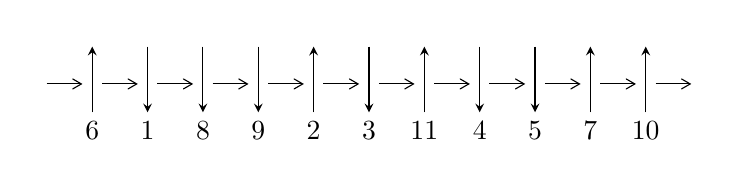
\begin{tikzpicture}[x=20pt, y=17pt]
	% nodes
	\node (C0) at (0, 0) {};
	\node (C1) at (1, 0) {};
	\node (C1U) at (1, +1) {};
	\node (C1D) at (1, -1) {6};

	\node (C2) at (2, 0) {};
	\node (C2U) at (2, +1) {};
	\node (C2D) at (2, -1) {1};

	\node (C3) at (3, 0) {};
	\node (C3U) at (3, +1) {};
	\node (C3D) at (3, -1) {8};

	\node (C4) at (4, 0) {};
	\node (C4U) at (4, +1) {};
	\node (C4D) at (4, -1) {9};

	\node (C5) at (5, 0) {};
	\node (C5U) at (5, +1) {};
	\node (C5D) at (5, -1) {2};

	\node (C6) at (6, 0) {};
	\node (C6U) at (6, +1) {};
	\node (C6D) at (6, -1) {3};

	\node (C7) at (7, 0) {};
	\node (C7U) at (7, +1) {};
	\node (C7D) at (7, -1) {11};

	\node (C8) at (8, 0) {};
	\node (C8U) at (8, +1) {};
	\node (C8D) at (8, -1) {4};

	\node (C9) at (9, 0) {};
	\node (C9U) at (9, +1) {};
	\node (C9D) at (9, -1) {5};

	\node (C10) at (10, 0) {};
	\node (C10U) at (10, +1) {};
	\node (C10D) at (10, -1) {7};

	\node (C11) at (11, 0) {};
	\node (C11U) at (11, +1) {};
	\node (C11D) at (11, -1) {10};
	\node (C12) at (12, 0) {};

	% arrows
	\draw[->,>={angle 60}]
	(C0) edge (C1) (C1) edge (C2) (C2) edge (C3) (C3) edge (C4) (C4) edge (C5) (C5) edge (C6) (C6) edge (C7) (C7) edge (C8) (C8) edge (C9) (C9) edge (C10) (C10) edge (C11) (C11) edge (C12) ;	\draw[->,>=stealth]
	(C1D) edge (C1U) (C2U) edge (C2D) (C3U) edge (C3D) (C4U) edge (C4D) (C5D) edge (C5U) (C6U) edge (C6D) (C7D) edge (C7U) (C8U) edge (C8D) (C9U) edge (C9D) (C10D) edge (C10U) (C11D) edge (C11U) ;
	\end{tikzpicture} \\
\hhline{~~} \\& 
\textbf{Solving Sequence} \\ \cline{2-2} 
 &
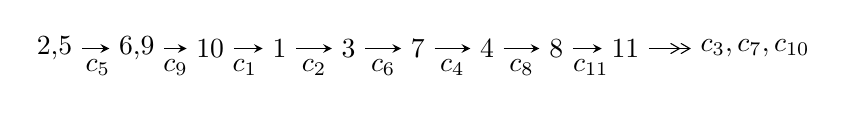
\begin{tikzpicture}[x=25pt, y=7pt]
	% node
	\node (A0) at (-1/8, 0) {2,5};
	\node (A1) at (17/16, 0) {6,9};
	\node (A2) at (17/8, 0) {10};
	\node (A3) at (25/8, 0) {1};
	\node (A4) at (33/8, 0) {3};
	\node (A5) at (41/8, 0) {7};
	\node (A6) at (49/8, 0) {4};
	\node (A7) at (57/8, 0) {8};
	\node (A8) at (65/8, 0) {11};
	\node (C1) at (1/2, -1) {$c_{5}$};
	\node (C2) at (13/8, -1) {$c_{9}$};
	\node (C3) at (21/8, -1) {$c_{1}$};
	\node (C4) at (29/8, -1) {$c_{2}$};
	\node (C5) at (37/8, -1) {$c_{6}$};
	\node (C6) at (45/8, -1) {$c_{4}$};
	\node (C7) at (53/8, -1) {$c_{8}$};
	\node (C8) at (61/8, -1) {$c_{11}$};
	\node (A9) at (10, 0) {$c_{3},c_{7},c_{10}$};

	% edge
	\draw[->,>=stealth]	
	(A0) edge (A1) (A1) edge (A2) (A2) edge (A3) (A3) edge (A4) (A4) edge (A5) (A5) edge (A6) (A6) edge (A7) (A7) edge (A8) ;
	\draw[->>,>={angle 60}]	
	(A8) edge (A9);
\end{tikzpicture} \\ 

\end{tabular} \\

\footnotetext{
The image of knot diagram is generated by the software ``\textbf{Draw programme}" developed by Andrew Bartholomew(\url{http://www.layer8.co.uk/maths/draw/index.htm\#Running-draw}), where we modified some parts for our purpose(\url{https://github.com/CATsTAILs/LinksPainter}).
}\phantom \\ \newline 
\centering \textbf{Ideals for irreducible components\footnotemark of $X_{\text{par}}$} 
 
\begin{align*}
I^u_{1}&=\langle 
-1.06825\times10^{16} u^{50}+1.14118\times10^{17} u^{49}+\cdots+1.72441\times10^{17} b+1.78982\times10^{17},\\
\phantom{I^u_{1}}&\phantom{= \langle  }1.65108\times10^{17} u^{50}-3.23686\times10^{17} u^{49}+\cdots+1.72441\times10^{17} a+6.56927\times10^{17},\;u^{51}-2 u^{50}+\cdots+2 u-1\rangle \\
I^u_{2}&=\langle 
- a u+b- a-1,\;a^2-2 a u+u+1,\;u^2+u+1\rangle \\
I^u_{3}&=\langle 
b,\;a- u,\;u^2- u+1\rangle \\
\\
\end{align*}
\raggedright * 3 irreducible components of $\dim_{\mathbb{C}}=0$, with total 57 representations.\\
\footnotetext{All coefficients of polynomials are rational numbers. But the coefficients are sometimes approximated in decimal forms when there is not enough margin.}
\newpage
\renewcommand{\arraystretch}{1}
\centering \section*{I. $I^u_{1}= \langle -1.07\times10^{16} u^{50}+1.14\times10^{17} u^{49}+\cdots+1.72\times10^{17} b+1.79\times10^{17},\;1.65\times10^{17} u^{50}-3.24\times10^{17} u^{49}+\cdots+1.72\times10^{17} a+6.57\times10^{17},\;u^{51}-2 u^{50}+\cdots+2 u-1 \rangle$}
\flushleft \textbf{(i) Arc colorings}\\
\begin{tabular}{m{7pt} m{180pt} m{7pt} m{180pt} }
\flushright $a_{2}=$&$\begin{pmatrix}0\\u\end{pmatrix}$ \\
\flushright $a_{5}=$&$\begin{pmatrix}1\\0\end{pmatrix}$ \\
\flushright $a_{6}=$&$\begin{pmatrix}1\\- u^2\end{pmatrix}$ \\
\flushright $a_{9}=$&$\begin{pmatrix}-0.957478 u^{50}+1.87709 u^{49}+\cdots+6.34747 u-3.80958\\0.0619485 u^{50}-0.661781 u^{49}+\cdots-0.419204 u-1.03793\end{pmatrix}$ \\
\flushright $a_{10}=$&$\begin{pmatrix}-1.01943 u^{50}+2.53887 u^{49}+\cdots+6.76667 u-2.77164\\0.0619485 u^{50}-0.661781 u^{49}+\cdots-0.419204 u-1.03793\end{pmatrix}$ \\
\flushright $a_{1}=$&$\begin{pmatrix}- u\\u^3+u\end{pmatrix}$ \\
\flushright $a_{3}=$&$\begin{pmatrix}- u^3\\u^5+u^3+u\end{pmatrix}$ \\
\flushright $a_{7}=$&$\begin{pmatrix}- u^6- u^4+1\\u^8+2 u^6+2 u^4\end{pmatrix}$ \\
\flushright $a_{4}=$&$\begin{pmatrix}0.197966 u^{50}+0.121740 u^{49}+\cdots+6.34202 u-3.22404\\0.475917 u^{50}-0.906399 u^{49}+\cdots-1.37093 u-1.53340\end{pmatrix}$ \\
\flushright $a_{8}=$&$\begin{pmatrix}1.37822 u^{50}-3.01777 u^{49}+\cdots-6.77353 u+2.71826\\0.314717 u^{50}+0.217072 u^{49}+\cdots+1.51590 u+0.995630\end{pmatrix}$ \\
\flushright $a_{11}=$&$\begin{pmatrix}-1.28901 u^{50}+2.47244 u^{49}+\cdots+6.66242 u-3.49712\\-0.225525 u^{50}-0.324327 u^{49}+\cdots-0.729101 u-1.01135\end{pmatrix}$\\ \flushright $a_{11}=$&$\begin{pmatrix}-1.28901 u^{50}+2.47244 u^{49}+\cdots+6.66242 u-3.49712\\-0.225525 u^{50}-0.324327 u^{49}+\cdots-0.729101 u-1.01135\end{pmatrix}$\\&\end{tabular}
\flushleft \textbf{(ii) Obstruction class $= -1$}\\~\\
\flushleft \textbf{(iii) Cusp Shapes $= \frac{159651415798743733}{86220451832092937} u^{50}-\frac{251339651139007465}{86220451832092937} u^{49}+\cdots-\frac{382063726346780762}{86220451832092937} u-\frac{177790526868945837}{86220451832092937}$}\\~\\
\newpage\renewcommand{\arraystretch}{1}
\flushleft \textbf{(iv) u-Polynomials at the component}\newline \\
\begin{tabular}{m{50pt}|m{274pt}}
Crossings & \hspace{64pt}u-Polynomials at each crossing \\
\hline $$\begin{aligned}c_{1},c_{5}\end{aligned}$$&$\begin{aligned}
&u^{51}-2 u^{50}+\cdots+2 u-1
\end{aligned}$\\
\hline $$\begin{aligned}c_{2}\end{aligned}$$&$\begin{aligned}
&u^{51}+26 u^{50}+\cdots-4 u-1
\end{aligned}$\\
\hline $$\begin{aligned}c_{3},c_{4},c_{8}\\c_{9}\end{aligned}$$&$\begin{aligned}
&u^{51}- u^{50}+\cdots+12 u+4
\end{aligned}$\\
\hline $$\begin{aligned}c_{6}\end{aligned}$$&$\begin{aligned}
&u^{51}+2 u^{50}+\cdots+102 u-289
\end{aligned}$\\
\hline $$\begin{aligned}c_{7},c_{10}\end{aligned}$$&$\begin{aligned}
&u^{51}-3 u^{50}+\cdots- u+7
\end{aligned}$\\
\hline $$\begin{aligned}c_{11}\end{aligned}$$&$\begin{aligned}
&u^{51}-23 u^{50}+\cdots+85 u-49
\end{aligned}$\\
\hline
\end{tabular}\\~\\
\newpage\renewcommand{\arraystretch}{1}
\flushleft \textbf{(v) Riley Polynomials at the component}\newline \\
\begin{tabular}{m{50pt}|m{274pt}}
Crossings & \hspace{64pt}Riley Polynomials at each crossing \\
\hline $$\begin{aligned}c_{1},c_{5}\end{aligned}$$&$\begin{aligned}
&y^{51}+26 y^{50}+\cdots-4 y-1
\end{aligned}$\\
\hline $$\begin{aligned}c_{2}\end{aligned}$$&$\begin{aligned}
&y^{51}+2 y^{50}+\cdots+20 y-1
\end{aligned}$\\
\hline $$\begin{aligned}c_{3},c_{4},c_{8}\\c_{9}\end{aligned}$$&$\begin{aligned}
&y^{51}-61 y^{50}+\cdots+208 y-16
\end{aligned}$\\
\hline $$\begin{aligned}c_{6}\end{aligned}$$&$\begin{aligned}
&y^{51}-22 y^{50}+\cdots-130628 y-83521
\end{aligned}$\\
\hline $$\begin{aligned}c_{7},c_{10}\end{aligned}$$&$\begin{aligned}
&y^{51}-23 y^{50}+\cdots+85 y-49
\end{aligned}$\\
\hline $$\begin{aligned}c_{11}\end{aligned}$$&$\begin{aligned}
&y^{51}+17 y^{50}+\cdots+63869 y-2401
\end{aligned}$\\
\hline
\end{tabular}\\~\\
\newpage\flushleft \textbf{(vi) Complex Volumes and Cusp Shapes}
$$\begin{array}{c|c|c}  
\text{Solutions to }I^u_{1}& \I (\text{vol} + \sqrt{-1}CS) & \text{Cusp shape}\\
 \hline 
\begin{aligned}
u &= \phantom{-}0.653226 + 0.692698 I \\
a &= -0.148299 + 0.771802 I \\
b &= \phantom{-}0.548925 - 0.344769 I\end{aligned}
 & \phantom{-}1.91333 + 3.68884 I & -0.17566 - 8.64084 I \\ \hline\begin{aligned}
u &= \phantom{-}0.653226 - 0.692698 I \\
a &= -0.148299 - 0.771802 I \\
b &= \phantom{-}0.548925 + 0.344769 I\end{aligned}
 & \phantom{-}1.91333 - 3.68884 I & -0.17566 + 8.64084 I \\ \hline\begin{aligned}
u &= -0.373145 + 0.994821 I \\
a &= \phantom{-}1.14320 - 1.08432 I \\
b &= \phantom{-}1.269780 + 0.040551 I\end{aligned}
 & -4.95677 - 2.83280 I & -9.17472 + 5.31542 I \\ \hline\begin{aligned}
u &= -0.373145 - 0.994821 I \\
a &= \phantom{-}1.14320 + 1.08432 I \\
b &= \phantom{-}1.269780 - 0.040551 I\end{aligned}
 & -4.95677 + 2.83280 I & -9.17472 - 5.31542 I \\ \hline\begin{aligned}
u &= -0.761774 + 0.749195 I \\
a &= -0.278985 + 1.056910 I \\
b &= -1.57317 - 0.07465 I\end{aligned}
 & -5.34945 - 5.09088 I & -4.00636 + 5.74458 I \\ \hline\begin{aligned}
u &= -0.761774 - 0.749195 I \\
a &= -0.278985 - 1.056910 I \\
b &= -1.57317 + 0.07465 I\end{aligned}
 & -5.34945 + 5.09088 I & -4.00636 - 5.74458 I \\ \hline\begin{aligned}
u &= \phantom{-}0.873962 + 0.290660 I \\
a &= -0.558370 + 0.726636 I \\
b &= -1.61853 - 0.15433 I\end{aligned}
 & -8.11783 - 8.19112 I & -3.54072 + 4.45146 I \\ \hline\begin{aligned}
u &= \phantom{-}0.873962 - 0.290660 I \\
a &= -0.558370 - 0.726636 I \\
b &= -1.61853 + 0.15433 I\end{aligned}
 & -8.11783 + 8.19112 I & -3.54072 - 4.45146 I \\ \hline\begin{aligned}
u &= \phantom{-}0.606693 + 0.904521 I \\
a &= \phantom{-}0.425610 - 0.192324 I \\
b &= -0.478539 - 0.218508 I\end{aligned}
 & \phantom{-}1.29833 + 1.21266 I & -3.42209 + 3.60169 I \\ \hline\begin{aligned}
u &= \phantom{-}0.606693 - 0.904521 I \\
a &= \phantom{-}0.425610 + 0.192324 I \\
b &= -0.478539 + 0.218508 I\end{aligned}
 & \phantom{-}1.29833 - 1.21266 I & -3.42209 - 3.60169 I\\
 \hline 
 \end{array}$$\newpage$$\begin{array}{c|c|c}  
\text{Solutions to }I^u_{1}& \I (\text{vol} + \sqrt{-1}CS) & \text{Cusp shape}\\
 \hline 
\begin{aligned}
u &= -0.477844 + 1.005770 I \\
a &= -1.81776 + 1.00351 I \\
b &= -0.550123 - 0.216418 I\end{aligned}
 & \phantom{-}1.10277 - 2.92056 I & -4.16055 + 6.87287 I \\ \hline\begin{aligned}
u &= -0.477844 - 1.005770 I \\
a &= -1.81776 - 1.00351 I \\
b &= -0.550123 + 0.216418 I\end{aligned}
 & \phantom{-}1.10277 + 2.92056 I & -4.16055 - 6.87287 I \\ \hline\begin{aligned}
u &= \phantom{-}0.848872 + 0.178353 I \\
a &= \phantom{-}0.815584 - 0.510581 I \\
b &= \phantom{-}1.63006 + 0.09121 I\end{aligned}
 & -10.01400 - 2.30364 I & -5.81940 + 0.26148 I \\ \hline\begin{aligned}
u &= \phantom{-}0.848872 - 0.178353 I \\
a &= \phantom{-}0.815584 + 0.510581 I \\
b &= \phantom{-}1.63006 - 0.09121 I\end{aligned}
 & -10.01400 + 2.30364 I & -5.81940 - 0.26148 I \\ \hline\begin{aligned}
u &= -0.715111 + 0.887420 I \\
a &= \phantom{-}0.440048 - 0.989396 I \\
b &= \phantom{-}1.56489 - 0.03455 I\end{aligned}
 & -5.76367 - 0.45170 I & -5.30593 + 0. I\phantom{ +0.000000I} \\ \hline\begin{aligned}
u &= -0.715111 - 0.887420 I \\
a &= \phantom{-}0.440048 + 0.989396 I \\
b &= \phantom{-}1.56489 + 0.03455 I\end{aligned}
 & -5.76367 + 0.45170 I & -5.30593 + 0. I\phantom{ +0.000000I} \\ \hline\begin{aligned}
u &= \phantom{-}0.385624 + 1.094960 I \\
a &= -0.487613 - 0.077571 I \\
b &= -0.003368 + 0.682499 I\end{aligned}
 & -1.93767 + 1.33394 I & -3.91651 + 0. I\phantom{ +0.000000I} \\ \hline\begin{aligned}
u &= \phantom{-}0.385624 - 1.094960 I \\
a &= -0.487613 + 0.077571 I \\
b &= -0.003368 - 0.682499 I\end{aligned}
 & -1.93767 - 1.33394 I & -3.91651 + 0. I\phantom{ +0.000000I} \\ \hline\begin{aligned}
u &= -0.777418 + 0.276187 I \\
a &= \phantom{-}0.106054 + 0.767256 I \\
b &= \phantom{-}0.725460 - 0.523141 I\end{aligned}
 & -0.15019 + 5.64266 I & -1.04154 - 6.14060 I \\ \hline\begin{aligned}
u &= -0.777418 - 0.276187 I \\
a &= \phantom{-}0.106054 - 0.767256 I \\
b &= \phantom{-}0.725460 + 0.523141 I\end{aligned}
 & -0.15019 - 5.64266 I & -1.04154 + 6.14060 I\\
 \hline 
 \end{array}$$\newpage$$\begin{array}{c|c|c}  
\text{Solutions to }I^u_{1}& \I (\text{vol} + \sqrt{-1}CS) & \text{Cusp shape}\\
 \hline 
\begin{aligned}
u &= -0.393138 + 1.114690 I \\
a &= \phantom{-}1.037440 - 0.580996 I \\
b &= \phantom{-}1.049420 - 0.251699 I\end{aligned}
 & -5.15851 - 2.68412 I & -8.38581 + 3.33159 I \\ \hline\begin{aligned}
u &= -0.393138 - 1.114690 I \\
a &= \phantom{-}1.037440 + 0.580996 I \\
b &= \phantom{-}1.049420 + 0.251699 I\end{aligned}
 & -5.15851 + 2.68412 I & -8.38581 - 3.33159 I \\ \hline\begin{aligned}
u &= -0.282693 + 1.153160 I \\
a &= -0.980168 + 0.289348 I \\
b &= -0.854041 + 0.456398 I\end{aligned}
 & -4.54342 + 2.50022 I & -7.39422 - 3.48023 I \\ \hline\begin{aligned}
u &= -0.282693 - 1.153160 I \\
a &= -0.980168 - 0.289348 I \\
b &= -0.854041 - 0.456398 I\end{aligned}
 & -4.54342 - 2.50022 I & -7.39422 + 3.48023 I \\ \hline\begin{aligned}
u &= \phantom{-}0.452176 + 1.119860 I \\
a &= \phantom{-}3.26876 + 1.81417 I \\
b &= \phantom{-}1.58540 - 0.04944 I\end{aligned}
 & -6.32061 + 3.82021 I & \phantom{-0.000000 } 0 \\ \hline\begin{aligned}
u &= \phantom{-}0.452176 - 1.119860 I \\
a &= \phantom{-}3.26876 - 1.81417 I \\
b &= \phantom{-}1.58540 + 0.04944 I\end{aligned}
 & -6.32061 - 3.82021 I & \phantom{-0.000000 } 0 \\ \hline\begin{aligned}
u &= \phantom{-}0.503800 + 1.120900 I \\
a &= \phantom{-}0.470374 + 0.032521 I \\
b &= -0.202005 - 0.728941 I\end{aligned}
 & -1.07037 + 6.18731 I & \phantom{-0.000000 } 0 \\ \hline\begin{aligned}
u &= \phantom{-}0.503800 - 1.120900 I \\
a &= \phantom{-}0.470374 - 0.032521 I \\
b &= -0.202005 + 0.728941 I\end{aligned}
 & -1.07037 - 6.18731 I & \phantom{-0.000000 } 0 \\ \hline\begin{aligned}
u &= -0.484334 + 1.137730 I \\
a &= \phantom{-}1.38555 - 0.92980 I \\
b &= \phantom{-}0.839056 + 0.455492 I\end{aligned}
 & -4.51627 - 5.12379 I & \phantom{-0.000000 } 0 \\ \hline\begin{aligned}
u &= -0.484334 - 1.137730 I \\
a &= \phantom{-}1.38555 + 0.92980 I \\
b &= \phantom{-}0.839056 - 0.455492 I\end{aligned}
 & -4.51627 + 5.12379 I & \phantom{-0.000000 } 0\\
 \hline 
 \end{array}$$\newpage$$\begin{array}{c|c|c}  
\text{Solutions to }I^u_{1}& \I (\text{vol} + \sqrt{-1}CS) & \text{Cusp shape}\\
 \hline 
\begin{aligned}
u &= \phantom{-}0.269126 + 0.708216 I \\
a &= -0.449611 - 0.544666 I \\
b &= -0.265341 + 0.389045 I\end{aligned}
 & -0.326016 + 1.158490 I & -3.80255 - 5.96760 I \\ \hline\begin{aligned}
u &= \phantom{-}0.269126 - 0.708216 I \\
a &= -0.449611 + 0.544666 I \\
b &= -0.265341 - 0.389045 I\end{aligned}
 & -0.326016 - 1.158490 I & -3.80255 + 5.96760 I \\ \hline\begin{aligned}
u &= -0.468235 + 0.565840 I \\
a &= \phantom{-}0.731516 + 1.135060 I \\
b &= \phantom{-}0.363476 - 0.377017 I\end{aligned}
 & \phantom{-}2.43662 - 1.03982 I & \phantom{-}2.70309 - 2.37854 I \\ \hline\begin{aligned}
u &= -0.468235 - 0.565840 I \\
a &= \phantom{-}0.731516 - 1.135060 I \\
b &= \phantom{-}0.363476 + 0.377017 I\end{aligned}
 & \phantom{-}2.43662 + 1.03982 I & \phantom{-}2.70309 + 2.37854 I \\ \hline\begin{aligned}
u &= \phantom{-}0.241188 + 1.242520 I \\
a &= \phantom{-}2.55925 + 0.13213 I \\
b &= \phantom{-}1.65434 + 0.12357 I\end{aligned}
 & -13.17000 - 4.70678 I & \phantom{-0.000000 } 0 \\ \hline\begin{aligned}
u &= \phantom{-}0.241188 - 1.242520 I \\
a &= \phantom{-}2.55925 - 0.13213 I \\
b &= \phantom{-}1.65434 - 0.12357 I\end{aligned}
 & -13.17000 + 4.70678 I & \phantom{-0.000000 } 0 \\ \hline\begin{aligned}
u &= -0.551420 + 1.150110 I \\
a &= -1.29108 + 0.99248 I \\
b &= -0.754244 - 0.593767 I\end{aligned}
 & -2.72526 - 10.62070 I & \phantom{-0.000000 } 0 \\ \hline\begin{aligned}
u &= -0.551420 - 1.150110 I \\
a &= -1.29108 - 0.99248 I \\
b &= -0.754244 + 0.593767 I\end{aligned}
 & -2.72526 + 10.62070 I & \phantom{-0.000000 } 0 \\ \hline\begin{aligned}
u &= \phantom{-}0.330757 + 1.237090 I \\
a &= -2.64813 - 0.57334 I \\
b &= -1.67128 - 0.05432 I\end{aligned}
 & -14.4656 + 1.6283 I & \phantom{-0.000000 } 0 \\ \hline\begin{aligned}
u &= \phantom{-}0.330757 - 1.237090 I \\
a &= -2.64813 + 0.57334 I \\
b &= -1.67128 + 0.05432 I\end{aligned}
 & -14.4656 - 1.6283 I & \phantom{-0.000000 } 0\\
 \hline 
 \end{array}$$\newpage$$\begin{array}{c|c|c}  
\text{Solutions to }I^u_{1}& \I (\text{vol} + \sqrt{-1}CS) & \text{Cusp shape}\\
 \hline 
\begin{aligned}
u &= \phantom{-}0.533489 + 1.196450 I \\
a &= -2.19793 - 1.79578 I \\
b &= -1.64958 + 0.12738 I\end{aligned}
 & -13.0576 + 7.3517 I & \phantom{-0.000000 } 0 \\ \hline\begin{aligned}
u &= \phantom{-}0.533489 - 1.196450 I \\
a &= -2.19793 + 1.79578 I \\
b &= -1.64958 - 0.12738 I\end{aligned}
 & -13.0576 - 7.3517 I & \phantom{-0.000000 } 0 \\ \hline\begin{aligned}
u &= \phantom{-}0.585702 + 1.179630 I \\
a &= \phantom{-}1.87475 + 2.03032 I \\
b &= \phantom{-}1.62902 - 0.17990 I\end{aligned}
 & -10.7944 + 13.5574 I & \phantom{-0.000000 } 0 \\ \hline\begin{aligned}
u &= \phantom{-}0.585702 - 1.179630 I \\
a &= \phantom{-}1.87475 - 2.03032 I \\
b &= \phantom{-}1.62902 + 0.17990 I\end{aligned}
 & -10.7944 - 13.5574 I & \phantom{-0.000000 } 0 \\ \hline\begin{aligned}
u &= -0.658054 + 0.143633 I \\
a &= -0.156833 - 0.508796 I \\
b &= -0.772507 + 0.296101 I\end{aligned}
 & -1.73343 + 0.77952 I & -4.48847 - 1.15850 I \\ \hline\begin{aligned}
u &= -0.658054 - 0.143633 I \\
a &= -0.156833 + 0.508796 I \\
b &= -0.772507 - 0.296101 I\end{aligned}
 & -1.73343 - 0.77952 I & -4.48847 + 1.15850 I \\ \hline\begin{aligned}
u &= \phantom{-}0.624363 + 0.237680 I \\
a &= \phantom{-}0.082181 + 1.030970 I \\
b &= \phantom{-}0.193282 - 0.611091 I\end{aligned}
 & \phantom{-}1.42567 - 1.76270 I & \phantom{-}2.33352 + 1.54024 I \\ \hline\begin{aligned}
u &= \phantom{-}0.624363 - 0.237680 I \\
a &= \phantom{-}0.082181 - 1.030970 I \\
b &= \phantom{-}0.193282 + 0.611091 I\end{aligned}
 & \phantom{-}1.42567 + 1.76270 I & \phantom{-}2.33352 - 1.54024 I \\ \hline\begin{aligned}
u &= -0.207283 + 0.506525 I \\
a &= -0.41811 + 2.77427 I \\
b &= -1.406490 - 0.077528 I\end{aligned}
 & -3.26856 - 0.24799 I & -3.08378 - 1.55453 I \\ \hline\begin{aligned}
u &= -0.207283 - 0.506525 I \\
a &= -0.41811 - 2.77427 I \\
b &= -1.406490 + 0.077528 I\end{aligned}
 & -3.26856 + 0.24799 I & -3.08378 + 1.55453 I\\
 \hline 
 \end{array}$$\newpage$$\begin{array}{c|c|c}  
\text{Solutions to }I^u_{1}& \I (\text{vol} + \sqrt{-1}CS) & \text{Cusp shape}\\
 \hline 
\begin{aligned}
u &= \phantom{-}0.482939\phantom{ +0.000000I} \\
a &= -2.81485\phantom{ +0.000000I} \\
b &= -1.50782\phantom{ +0.000000I}\end{aligned}
 & -3.54033\phantom{ +0.000000I} & -1.57180\phantom{ +0.000000I}\\
 \hline 
 \end{array}$$\newpage\newpage\renewcommand{\arraystretch}{1}
\centering \section*{II. $I^u_{2}= \langle - a u+b- a-1,\;a^2-2 a u+u+1,\;u^2+u+1 \rangle$}
\flushleft \textbf{(i) Arc colorings}\\
\begin{tabular}{m{7pt} m{180pt} m{7pt} m{180pt} }
\flushright $a_{2}=$&$\begin{pmatrix}0\\u\end{pmatrix}$ \\
\flushright $a_{5}=$&$\begin{pmatrix}1\\0\end{pmatrix}$ \\
\flushright $a_{6}=$&$\begin{pmatrix}1\\u+1\end{pmatrix}$ \\
\flushright $a_{9}=$&$\begin{pmatrix}a\\a u+a+1\end{pmatrix}$ \\
\flushright $a_{10}=$&$\begin{pmatrix}- a u-1\\a u+a+1\end{pmatrix}$ \\
\flushright $a_{1}=$&$\begin{pmatrix}- u\\u+1\end{pmatrix}$ \\
\flushright $a_{3}=$&$\begin{pmatrix}-1\\0\end{pmatrix}$ \\
\flushright $a_{7}=$&$\begin{pmatrix}- u\\u+1\end{pmatrix}$ \\
\flushright $a_{4}=$&$\begin{pmatrix}a+u+1\\-2\end{pmatrix}$ \\
\flushright $a_{8}=$&$\begin{pmatrix}a u+1\\- a u- a-1\end{pmatrix}$ \\
\flushright $a_{11}=$&$\begin{pmatrix}- a u- u-1\\a u+a+u+2\end{pmatrix}$\\ \flushright $a_{11}=$&$\begin{pmatrix}- a u- u-1\\a u+a+u+2\end{pmatrix}$\\&\end{tabular}
\flushleft \textbf{(ii) Obstruction class $= 1$}\\~\\
\flushleft \textbf{(iii) Cusp Shapes $= 4 u$}\\~\\
\newpage\renewcommand{\arraystretch}{1}
\flushleft \textbf{(iv) u-Polynomials at the component}\newline \\
\begin{tabular}{m{50pt}|m{274pt}}
Crossings & \hspace{64pt}u-Polynomials at each crossing \\
\hline $$\begin{aligned}c_{1},c_{6}\end{aligned}$$&$\begin{aligned}
&(u^2- u+1)^2
\end{aligned}$\\
\hline $$\begin{aligned}c_{2},c_{5}\end{aligned}$$&$\begin{aligned}
&(u^2+u+1)^2
\end{aligned}$\\
\hline $$\begin{aligned}c_{3},c_{4},c_{8}\\c_{9}\end{aligned}$$&$\begin{aligned}
&(u^2-2)^2
\end{aligned}$\\
\hline $$\begin{aligned}c_{7},c_{11}\end{aligned}$$&$\begin{aligned}
&(u-1)^4
\end{aligned}$\\
\hline $$\begin{aligned}c_{10}\end{aligned}$$&$\begin{aligned}
&(u+1)^4
\end{aligned}$\\
\hline
\end{tabular}\\~\\
\newpage\renewcommand{\arraystretch}{1}
\flushleft \textbf{(v) Riley Polynomials at the component}\newline \\
\begin{tabular}{m{50pt}|m{274pt}}
Crossings & \hspace{64pt}Riley Polynomials at each crossing \\
\hline $$\begin{aligned}c_{1},c_{2},c_{5}\\c_{6}\end{aligned}$$&$\begin{aligned}
&(y^2+y+1)^2
\end{aligned}$\\
\hline $$\begin{aligned}c_{3},c_{4},c_{8}\\c_{9}\end{aligned}$$&$\begin{aligned}
&(y-2)^4
\end{aligned}$\\
\hline $$\begin{aligned}c_{7},c_{10},c_{11}\end{aligned}$$&$\begin{aligned}
&(y-1)^4
\end{aligned}$\\
\hline
\end{tabular}\\~\\
\newpage\flushleft \textbf{(vi) Complex Volumes and Cusp Shapes}
$$\begin{array}{c|c|c}  
\text{Solutions to }I^u_{2}& \I (\text{vol} + \sqrt{-1}CS) & \text{Cusp shape}\\
 \hline 
\begin{aligned}
u &= -0.500000 + 0.866025 I \\
a &= \phantom{-}0.207107 - 0.358719 I \\
b &= \phantom{-}1.41421\phantom{ +0.000000I}\end{aligned}
 & -3.28987 - 2.02988 I & -2.00000 + 3.46410 I \\ \hline\begin{aligned}
u &= -0.500000 + 0.866025 I \\
a &= -1.20711 + 2.09077 I \\
b &= -1.41421\phantom{ +0.000000I}\end{aligned}
 & -3.28987 - 2.02988 I & -2.00000 + 3.46410 I \\ \hline\begin{aligned}
u &= -0.500000 - 0.866025 I \\
a &= \phantom{-}0.207107 + 0.358719 I \\
b &= \phantom{-}1.41421\phantom{ +0.000000I}\end{aligned}
 & -3.28987 + 2.02988 I & -2.00000 - 3.46410 I \\ \hline\begin{aligned}
u &= -0.500000 - 0.866025 I \\
a &= -1.20711 - 2.09077 I \\
b &= -1.41421\phantom{ +0.000000I}\end{aligned}
 & -3.28987 + 2.02988 I & -2.00000 - 3.46410 I\\
 \hline 
 \end{array}$$\newpage\newpage\renewcommand{\arraystretch}{1}
\centering \section*{III. $I^u_{3}= \langle b,\;a- u,\;u^2- u+1 \rangle$}
\flushleft \textbf{(i) Arc colorings}\\
\begin{tabular}{m{7pt} m{180pt} m{7pt} m{180pt} }
\flushright $a_{2}=$&$\begin{pmatrix}0\\u\end{pmatrix}$ \\
\flushright $a_{5}=$&$\begin{pmatrix}1\\0\end{pmatrix}$ \\
\flushright $a_{6}=$&$\begin{pmatrix}1\\- u+1\end{pmatrix}$ \\
\flushright $a_{9}=$&$\begin{pmatrix}u\\0\end{pmatrix}$ \\
\flushright $a_{10}=$&$\begin{pmatrix}u\\0\end{pmatrix}$ \\
\flushright $a_{1}=$&$\begin{pmatrix}- u\\u-1\end{pmatrix}$ \\
\flushright $a_{3}=$&$\begin{pmatrix}1\\0\end{pmatrix}$ \\
\flushright $a_{7}=$&$\begin{pmatrix}u\\- u+1\end{pmatrix}$ \\
\flushright $a_{4}=$&$\begin{pmatrix}1\\0\end{pmatrix}$ \\
\flushright $a_{8}=$&$\begin{pmatrix}u\\0\end{pmatrix}$ \\
\flushright $a_{11}=$&$\begin{pmatrix}0\\u-1\end{pmatrix}$\\ \flushright $a_{11}=$&$\begin{pmatrix}0\\u-1\end{pmatrix}$\\&\end{tabular}
\flushleft \textbf{(ii) Obstruction class $= 1$}\\~\\
\flushleft \textbf{(iii) Cusp Shapes $= -4 u+2$}\\~\\
\newpage\renewcommand{\arraystretch}{1}
\flushleft \textbf{(iv) u-Polynomials at the component}\newline \\
\begin{tabular}{m{50pt}|m{274pt}}
Crossings & \hspace{64pt}u-Polynomials at each crossing \\
\hline $$\begin{aligned}c_{1},c_{2},c_{6}\end{aligned}$$&$\begin{aligned}
&u^2+u+1
\end{aligned}$\\
\hline $$\begin{aligned}c_{3},c_{4},c_{8}\\c_{9}\end{aligned}$$&$\begin{aligned}
&u^2
\end{aligned}$\\
\hline $$\begin{aligned}c_{5}\end{aligned}$$&$\begin{aligned}
&u^2- u+1
\end{aligned}$\\
\hline $$\begin{aligned}c_{7}\end{aligned}$$&$\begin{aligned}
&(u+1)^2
\end{aligned}$\\
\hline $$\begin{aligned}c_{10},c_{11}\end{aligned}$$&$\begin{aligned}
&(u-1)^2
\end{aligned}$\\
\hline
\end{tabular}\\~\\
\newpage\renewcommand{\arraystretch}{1}
\flushleft \textbf{(v) Riley Polynomials at the component}\newline \\
\begin{tabular}{m{50pt}|m{274pt}}
Crossings & \hspace{64pt}Riley Polynomials at each crossing \\
\hline $$\begin{aligned}c_{1},c_{2},c_{5}\\c_{6}\end{aligned}$$&$\begin{aligned}
&y^2+y+1
\end{aligned}$\\
\hline $$\begin{aligned}c_{3},c_{4},c_{8}\\c_{9}\end{aligned}$$&$\begin{aligned}
&y^2
\end{aligned}$\\
\hline $$\begin{aligned}c_{7},c_{10},c_{11}\end{aligned}$$&$\begin{aligned}
&(y-1)^2
\end{aligned}$\\
\hline
\end{tabular}\\~\\
\newpage\flushleft \textbf{(vi) Complex Volumes and Cusp Shapes}
$$\begin{array}{c|c|c}  
\text{Solutions to }I^u_{3}& \I (\text{vol} + \sqrt{-1}CS) & \text{Cusp shape}\\
 \hline 
\begin{aligned}
u &= \phantom{-}0.500000 + 0.866025 I \\
a &= \phantom{-}0.500000 + 0.866025 I \\
b &= \phantom{-0.000000 } 0\end{aligned}
 & \phantom{-}1.64493 + 2.02988 I & \phantom{-0.000000 } 0. - 3.46410 I \\ \hline\begin{aligned}
u &= \phantom{-}0.500000 - 0.866025 I \\
a &= \phantom{-}0.500000 - 0.866025 I \\
b &= \phantom{-0.000000 } 0\end{aligned}
 & \phantom{-}1.64493 - 2.02988 I & \phantom{-0.000000 -}0. + 3.46410 I\\
 \hline 
 \end{array}$$\newpage
\newpage\renewcommand{\arraystretch}{1}
\centering \section*{ IV. u-Polynomials}
\begin{tabular}{m{50pt}|m{274pt}}
Crossings & \hspace{64pt}u-Polynomials at each crossing \\
\hline $$\begin{aligned}c_{1}\end{aligned}$$&$\begin{aligned}
&((u^2- u+1)^2)(u^2+u+1)(u^{51}-2 u^{50}+\cdots+2 u-1)
\end{aligned}$\\
\hline $$\begin{aligned}c_{2}\end{aligned}$$&$\begin{aligned}
&((u^2+u+1)^3)(u^{51}+26 u^{50}+\cdots-4 u-1)
\end{aligned}$\\
\hline $$\begin{aligned}c_{3},c_{4},c_{8}\\c_{9}\end{aligned}$$&$\begin{aligned}
&u^2(u^2-2)^2(u^{51}- u^{50}+\cdots+12 u+4)
\end{aligned}$\\
\hline $$\begin{aligned}c_{5}\end{aligned}$$&$\begin{aligned}
&(u^2- u+1)(u^2+u+1)^2(u^{51}-2 u^{50}+\cdots+2 u-1)
\end{aligned}$\\
\hline $$\begin{aligned}c_{6}\end{aligned}$$&$\begin{aligned}
&((u^2- u+1)^2)(u^2+u+1)(u^{51}+2 u^{50}+\cdots+102 u-289)
\end{aligned}$\\
\hline $$\begin{aligned}c_{7}\end{aligned}$$&$\begin{aligned}
&((u-1)^4)(u+1)^2(u^{51}-3 u^{50}+\cdots- u+7)
\end{aligned}$\\
\hline $$\begin{aligned}c_{10}\end{aligned}$$&$\begin{aligned}
&((u-1)^2)(u+1)^4(u^{51}-3 u^{50}+\cdots- u+7)
\end{aligned}$\\
\hline $$\begin{aligned}c_{11}\end{aligned}$$&$\begin{aligned}
&((u-1)^6)(u^{51}-23 u^{50}+\cdots+85 u-49)
\end{aligned}$\\
\hline
\end{tabular}\newpage\renewcommand{\arraystretch}{1}
\centering \section*{ V. Riley Polynomials}
\begin{tabular}{m{50pt}|m{274pt}}
Crossings & \hspace{64pt}Riley Polynomials at each crossing \\
\hline $$\begin{aligned}c_{1},c_{5}\end{aligned}$$&$\begin{aligned}
&((y^2+y+1)^3)(y^{51}+26 y^{50}+\cdots-4 y-1)
\end{aligned}$\\
\hline $$\begin{aligned}c_{2}\end{aligned}$$&$\begin{aligned}
&((y^2+y+1)^3)(y^{51}+2 y^{50}+\cdots+20 y-1)
\end{aligned}$\\
\hline $$\begin{aligned}c_{3},c_{4},c_{8}\\c_{9}\end{aligned}$$&$\begin{aligned}
&y^2(y-2)^4(y^{51}-61 y^{50}+\cdots+208 y-16)
\end{aligned}$\\
\hline $$\begin{aligned}c_{6}\end{aligned}$$&$\begin{aligned}
&((y^2+y+1)^3)(y^{51}-22 y^{50}+\cdots-130628 y-83521)
\end{aligned}$\\
\hline $$\begin{aligned}c_{7},c_{10}\end{aligned}$$&$\begin{aligned}
&((y-1)^6)(y^{51}-23 y^{50}+\cdots+85 y-49)
\end{aligned}$\\
\hline $$\begin{aligned}c_{11}\end{aligned}$$&$\begin{aligned}
&((y-1)^6)(y^{51}+17 y^{50}+\cdots+63869 y-2401)
\end{aligned}$\\
\hline
\end{tabular}
\vskip 2pc
\end{document}